\chapter{Apartado B: \textbf{Filtro Gaussiano y Detección de bordes: Sobel y Canny}}
\label{chapter:tarea_b}

En este apartado, trabajará con filtros para procesar imágenes. Los conceptos clave de este apartado son:

\begin{itemize}
    \item \textbf{Filtro o Kernel}: es una matriz $n x n$ que se desliza de forma ordenada por la imagen. Según sus valores, un filtro puede servir para difuminar una imagen, extraer sus bordes, etc.
    \item \textbf{Convolución}. Es una operación matemática que en visión por ordenador sirve para modificar una imagen. Toma los valores del kernel y los de la imagen en la posición $(i, j)$ para producir el valor del píxel $(i, j)$ de la nueva imagen. \footnote{\href{https://gitlab.com/brohrer/convolution-2d-animation/-/tree/main}{Ejemplos animados de convoluciones}: https://gitlab.com/brohrer/convolution-2d-animation/-/tree/main}
    \item \textbf{Imagen}: El elemento sobre el que se aplica la operación.
\end{itemize}

Trabajará en la definición de tres filtros: Gausiano, Sobel y Canny. Una vez definidos, deberá aplicar cada uno de los filtros sobre las imágenes de la carpeta \texttt{data}. A continuación se añaden algunos comentarios para resolver la tarea:

\section*{Tarea B.1: Implementación de filtro Gausiano}
\phantomsection
\addcontentsline{toc}{section}{Tarea B.1: Implementación de filtro Gausiano}

Para aplicar el filtro Gausiano, deberá tener cuenta los siguientes factores:

\begin{itemize}
    \item \textbf{Tamaño del filtro}. Como podrá comprobar en los argumentos de la función, el tamaño del filtro puede (o no) venir dado. Cuando el tamaño del filtro no se pase como argumento, deberá obtener sus dimensiones a partir del valor de $\sigma$. Puede dar por supuesto que el efecto del filtro Gausiano se considera extinto más allá de $\pm4\sigma$. Además, tenga en cuenta que se busca un filtro $n x n$ donde $n$ es impar. La Figura \ref{fig:kernel_size} ilustra cómo aumenta el tamaño del filtro (\textit{kernel size}, K) cuando aumenta $\sigma$.

    \begin{figure}[h]
    \centering
    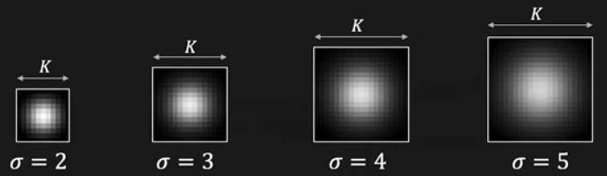
\includegraphics[width=0.6 \textwidth]{Lab_2/template/figures/kernel_size.png}
    \caption{Tamaño del kernel en función de $\sigma$.}
    \label{fig:kernel_size}
    \end{figure}

    Con las restricciones y condiciones mencionadas, deberá definir el tamaño del filtro de tal forma que se cumpla lo indicado en la Ecuación \ref{eq:kernel_size}:

    \begin{align}
     \text{shape} &= [L, L]\\
     L &= f(\sigma)
    \label{eq:kernel_size}
    \end{align}

    
    \item  \textbf{Coordenadas}. Con np.mgrid(), obtenga los valores de las coordenadas para $x$ e $y$ como dos arrays diferentes. Visite la documentación del método para visualizar un ejemplo de lo que se le pide.
    \item  \textbf{Fórmula}. Defina la fórmula del filtro Gausiano para cada elemento $(i, j)$ siguiendo la Ecuación \ref{eq:gausiano}.

    \begin{equation}
    G(i,j) = \frac{1}{\sigma \sqrt{2\pi}} e^{-\frac{1}{2} \left( \frac{i^2 + j^2}{\sigma^2} \right)}
    \label{eq:gausiano}
    \end{equation}

    \item  \textbf{Convolución}. Aplique sobre el argumento \texttt{img} la operación de convolución con el filtro que acaba de definir. Utilice el método de OpenCV \texttt{cv2.Filter2D()}.
\end{itemize}

\section*{Tarea B.2: Aplicación de filtro Gausiano}
\phantomsection
\addcontentsline{toc}{section}{Tarea B.2: Aplicación de filtro Gausiano}

Aplique el filtro que acaba de definir al conjunto de imágenes de la carpeta \texttt{data}. Defina las variables necesarias para llamar al método. Puede utilizar una \textit{list comprehension} para trabajar de forma eficiente. Como resultado de aplicar el filtro, debería obtener imágenes difuminadas o desenfocadas.

\section*{Tarea B.3: Implementación de filtro Sobel}
\phantomsection
\addcontentsline{toc}{section}{Tarea B.3: Implementación de filtro Sobel}

Para aplicar el filtro Sobel, deberá tener cuenta los siguientes factores:

\begin{itemize}
    \item \textbf{Imagen en escala de grises}. Trabaje con la imagen en escala de grises. Para ello, puede usar el método \texttt{cv2.cvtColor()} (que ya utilizó en la primera sesión de laboratorio).
    
    \item \textbf{Filtro Gausiano}. Utilice el método que ha definido anteriormente. Sea cuidadoso proporcionando cada argumento para que sea heredable (es decir, utilice variables como argumentos).
    
    \item \textbf{Bordes verticales}. Obtenga los bordes verticales utilizando el filtro dado (\texttt{filter}). De nuevo, utilice el método \texttt{cv2.Filter2D()}.
    \item \textbf{Transformación del filtro}. Transforme el filtro para obtener los bordes en la dirección ortogonal.
    \item \textbf{Bordes horizontales}. Con el filtro transformado, utilice de nuevo \texttt{cv2.Filter2D()} para obtener los bordes ortogonales.
    \item \textbf{Composición de bordes}. Obtenga los bordes de la imagen como una composición de los bordes detectados en cada dirección. Puede utilizar para ello \texttt{np.hypot()}.
    \item \textbf{Orientación}. Obtenga la orientación de los bordes con \texttt{np.arctan2()}.
\end{itemize}

\section*{Tarea B.4: Aplicación de filtro Sobel}
\phantomsection
\addcontentsline{toc}{section}{Tarea B.4: Aplicación de filtro Sobel}

Aplique el filtro que acaba de definir al conjunto de imágenes de la carpeta \texttt{data}. Defina las variables necesarias para llamar al método. Puede utilizar una \textit{list comprehension} para trabajar de forma eficiente. Como resultado de aplicar el filtro, debería obtener un resultado similar al de la Figura \ref{fig:edges}. El filtro que debe introducir como argumento de la función es:

\[
\begin{bmatrix}
-1 & 0 & 1 \\
-2 & 0 & 2 \\
-1 & 0 & 1
\end{bmatrix}
\]


\begin{figure}[H]
    \centering
    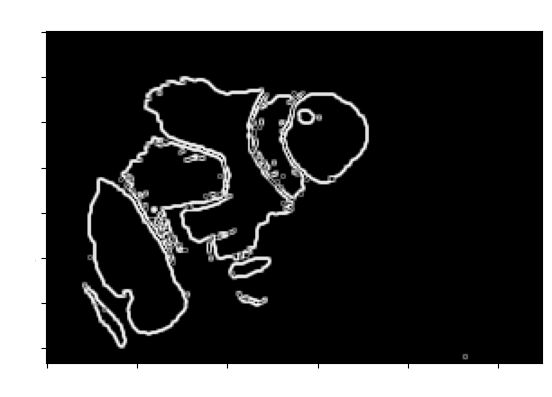
\includegraphics[width=0.3\textwidth]{Lab_2/template/figures/edges.png}
    \caption{Ejemplo de bordes detectados usando el filtro Sobel.}
    \label{fig:edges}
\end{figure}

\section*{Tarea B.5: Implementación de filtro Canny}
\phantomsection
\addcontentsline{toc}{section}{Tarea B.5: Implementación de filtro Canny}
El filtro Canny aporta un resultado más refinado para detectar bordes que el obtenido por Sobel. Para implementar el filtro Canny, deberá seguir los siguientes pasos:

\begin{itemize}
    \item \textbf{Filtro Sobel}. Realice una llamada al método del filtro Sobel que ha definido en los pasos anteriores. De nuevo,  sea cuidadoso proporcionando cada argumento para que sea heredable (es decir, utilice variables como argumentos).
    \item \textbf{Non Max Supresion}. Utilice el método \texttt{non\_max\_supression()} definido en el archivo \texttt{utils.py}. Inspeccione los argumentos que necesita utilizar este método para poder ejecutarlo de forma adecuada. Este método se encarga de refinar los bordes, devolviendo una imagen en escala de grises. 
\end{itemize}

\section*{Tarea B.6: Aplicación de filtro Canny}
\phantomsection
\addcontentsline{toc}{section}{Tarea B.6: Aplicación de filtro Canny}

Aplique el filtro que acaba de definir al conjunto de imágenes de la carpeta \texttt{data}. Defina las variables necesarias para llamar al método. Puede utilizar una \textit{list comprehension} para trabajar de forma eficiente. Como resultado de aplicar el filtro, debería obtener los bordes de las imágenes de forma similar a cuando aplicó el filtro Sobel.

\section*{Preguntas}
\addcontentsline{toc}{section}{Preguntas}

\vspace{5mm}
\begin{tcolorbox}[colback=gray!10, colframe=gray!30, coltitle=black, title=Pregunta B.1, halign=left]
Añada ruido a las imágenes de la carpeta \texttt{data}. Compare los resultados que obtiene al aplicar su filtro Sobel \textbf{con y sin filtro Gausiano}. Para añadir ruido, puede sumar a la imagen original una matriz de las dimensiones adecuadas. Puede utilizar \texttt{np.random.normal()}, pero tenga en cuenta que este proceso puede hacer que algunos valores de la imagen salgan del rango [0, 255] (tome las medidas necesarias para corregir esto).
\end{tcolorbox}

\vspace{5mm}
\begin{tcolorbox}[colback=gray!10, colframe=gray!30, coltitle=black, title=Pregunta B.2, halign=left]
Utilice la librería \texttt{scikit-image} y compare el efecto de los filtros Sobel, Canny y Prewitt sobre las imágenes de la carpeta \texttt{data}. ¿Qué diferencias observa entre los filtros? ¿Puede obtener alguna conclusión y/o patrón?
\end{tcolorbox}